\documentclass{ximera}

\title{The Idea of Limits}

\begin{document}
\begin{abstract}
This is a trial online lesson on an introduction to limits.
\end{abstract}
\maketitle

\section{Goals of this Lesson}
\subsection{Conceptual Goals:}

\begin{itemize}
\item Average velocity vs instaneous velocity
\item Secant live vs tangent line
\item What is a limit?
\end{itemize}

\subsection{Computational Goals:}

\begin{itemize}
\item Compute average velocity
\item Approximate instantaneous velocity
\item Calculus slope of a secant line
\end{itemize}


\section{Average Velocity}

\youtube{HwzVyIaiKcQ?autoplay=0&rel=0&end=97}

\begin{question}
  To find the average velocity over an interval, we should divide which two quantities?
  \begin{selectAll}
    \choice{The time when the interval ended}
    \choice{The final position of the ball}
    \choice[correct]{The length of time the interval lasted}
    \choice[correct]{The distance the ball traveled over the interval}
    \choice{The final speed of the ball}
    \choice{The intial position of the ball}
  \end{selectAll}
  \begin{feedback}
  The average velocity is the distance traveled divided by the length of the time interval.
  \end{feedback}
\end{question}


\begin{image}

\includegraphics{remember.png}
\end{image}
\begin{formula}
To find the average velocity:
\[
v_{av}=\frac{\text{change in position}}{\text{change in time}} = \frac{s(t_1)-s(t_0)}{t_1-t_0}
\]
where $s(t)$ is the position at time $t$ and the time interval $[t_0,t_1]$
\end{formula}

Practice Finding Average Velocity:
\begin{foldable}
\begin{image}
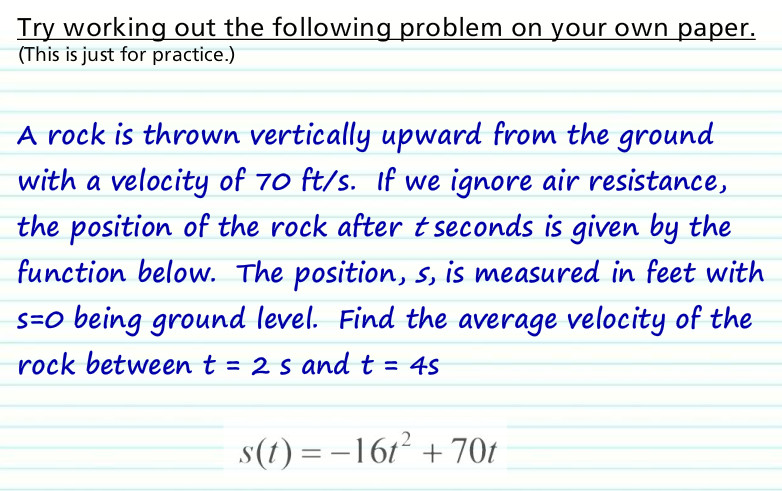
\includegraphics{picture1.png}
\end{image}

Click to see the solution:
\begin{foldable}
\begin{image}
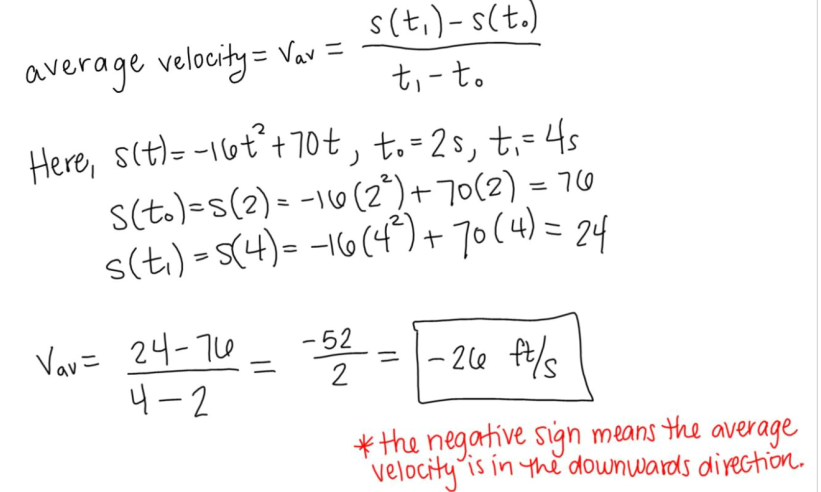
\includegraphics{picture2.png}
\end{image}
\end{foldable}
\end{foldable}

\youtube{HwzVyIaiKcQ?autoplay=98&rel=0&end=210}
 
\begin{question}
    Calculate the average velocity of the ball over the time interval $[1,2]$ for the position function shown below. 
    \begin{prompt}
        The average velocity is $\answer[given]{52}$.
    \end{prompt}
    
      \begin{feedback}
  The change in position is $s(2) - s(1) = 136 - 84 = 52$. The change in time is $2 - 1 = 1$.  Therefore, average velocity is $\frac{52}{1} = 52$.
  \end{feedback}
  
\end{question}

\begin{image}

\includegraphics{bigidea.png}
\end{image}
The average velocity changes if we use different intervals. \\
\textit{So...} \\
Average Velocity must be different from Instantaneous Velocity. \\
\textit{So...} \\
How do we find instantaneous velocity?


\section{Instantaneous Velocity}

\youtube{HwzVyIaiKcQ?autoplay=211&rel=0&end=720}

\begin{question}
  Which speed is the best estimate of the instantaneous velocity of the ball .4 seconds after it left Bart's hand? 
  \begin{multipleChoice}
    \choice{7 mph}
    \choice{8 mph}
    \choice[correct]{9 mph}
  \end{multipleChoice}
  \begin{feedback}
  The smaller the interval, the closer the average velocity is to the instantaneous velocity.
  \end{feedback}
\end{question}

\begin{image}
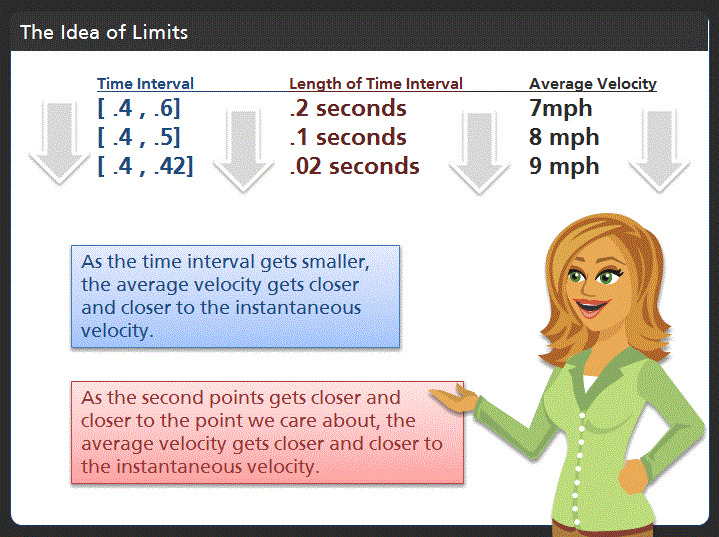
\includegraphics{picture3.png}
\end{image}

\youtube{HwzVyIaiKcQ?autoplay=720&rel=0&end=976}

\subsection{Optional Examples: Estimating instantaneous velocity}

Watch full length example:
\begin{foldable}
\youtube{7K437sKzLbM?autoplay=0&rel=0}
\end{foldable}

Watch shortened example: 
\begin{foldable}
\youtube{7K437sKzLbM?autoplay=0&rel=0&start=280}
\end{foldable}


\section{Secant Lines}

\begin{image}
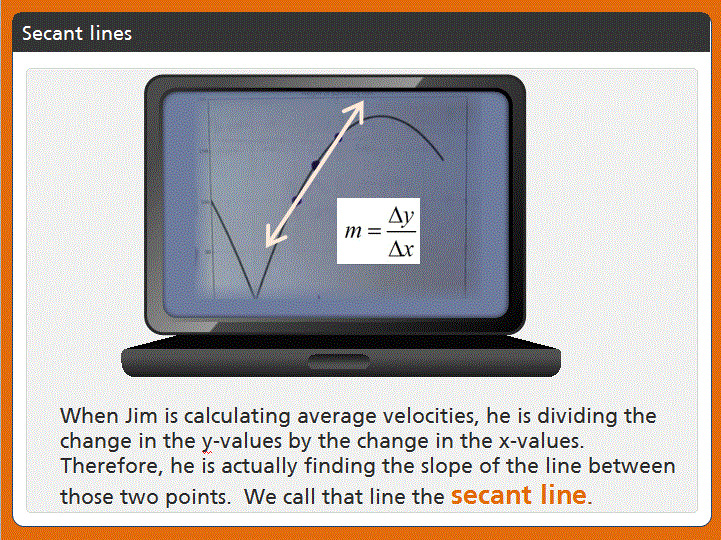
\includegraphics{picture4.png}
\end{image}

\youtube{QXUTiNNa68E?autoplay=0&rel=0&start=33&end=322}

\begin{image}
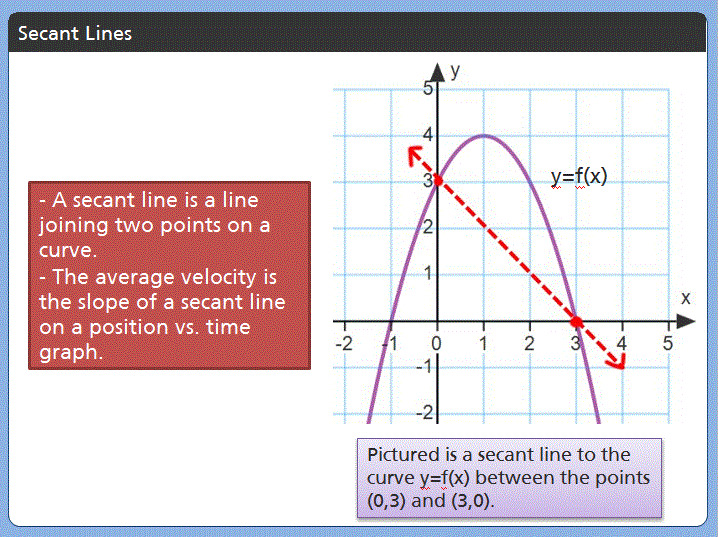
\includegraphics{picture5.png}
\end{image}

\section{Tangent Lines}

\youtube{XfnJbGmmVIA}

\begin{question}
  True or False. The tangent line is the line that connects two points on a curve. 
  \begin{multipleChoice}
    \choice{True}
    \choice[correct]{False}
  \end{multipleChoice}
  \begin{feedback}
  The secant line is the line that connects two points on a curve.
  \end{feedback}
\end{question}

\begin{image}
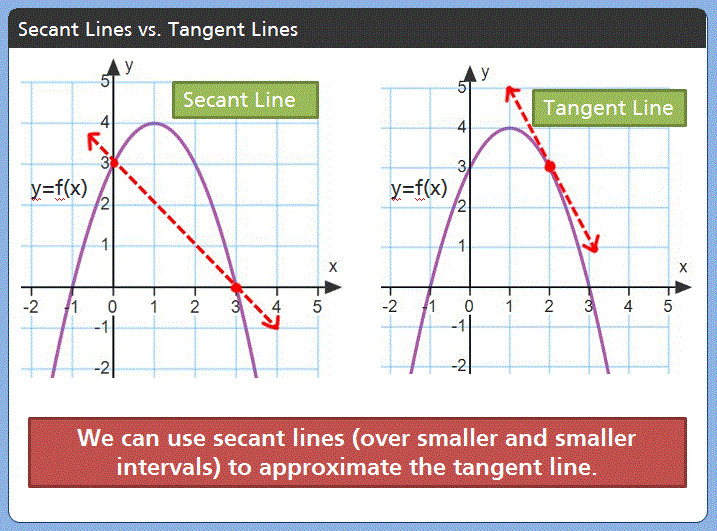
\includegraphics{picture6.png}
\end{image}

\subsection{Optional Examples: Estimating the slope of the tangent line}

Watch full length example:
\begin{foldable}
\youtube{__8Vag4OtAo?autoplay=0&rel=0}
\end{foldable}

Watch shortened example: 
\begin{foldable}
\youtube{__8Vag4OtAo?autoplay=0&rel=0&start=385}
\end{foldable}

\begin{image}

\includegraphics{bigidea.png}
\end{image}
To find the instantaneous velocity (the slope of the tangent line), we want our 2nd point to be as close to the point we care about as possible. \\
\textit{But...} \\
We cannot actually be at the point we care about because we need two points to find a slope (or we'd get 0/0). \\
\textit{So...} \\
This is why we need the mathematical idea of a LIMIT.

\begin{image}
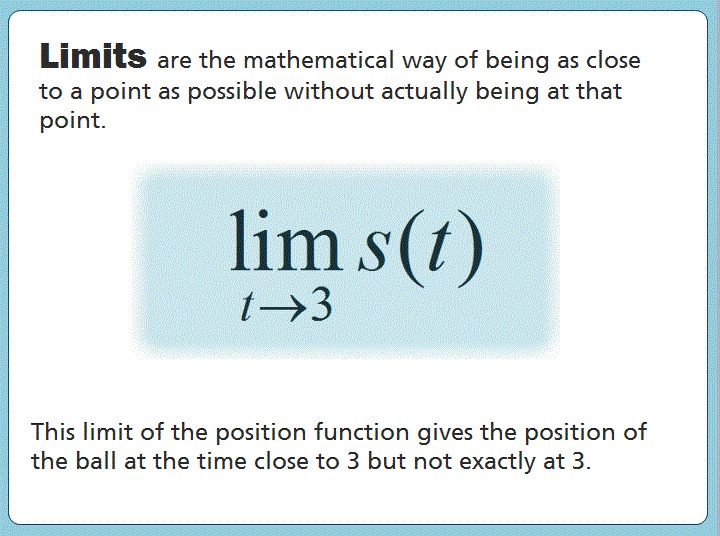
\includegraphics{picture7.png}
\end{image}

\youtube{HwzVyIaiKcQ?autoplay=0&rel=0&start=977}

\end{document}
